\appendix
\section{Retrospective single-receiver calibration diagnostic}\label{app:receiver}
To examine whether a fixed uncertainty envelope transfers across different time periods, we perform an exploratory diagnostic on the TST2 reference data from GraphGNSSLib~\citep{GraphGNSSData}. The sequence contains 157 matched reference epochs associated with precomputed RTKLIB 2.4.2 kinematic combined solutions. Horizontal east and north residuals are calculated relative to the reference coordinates supplied with the repository, without fitted alignment, bias correction, filtering, or interpolation. Vertical errors are excluded because the elevation datum and antenna-related conventions have not been established.

The first 78 epochs in chronological order are reserved for calibration, the next ten form a gap, and the final 69 are used for evaluation. If $e_j$ and $n_j$ are the east and north residuals at epoch $j$, define
\[
s_j=\max\bigl(|e_j|,|n_j|\bigr).
\]
The 76th ordered score among calibration epochs gives a square axis-aligned envelope with half-width 0.863506 m. We also test the east/north $3\sigma$ rectangular envelope reported by the original solution file. Table~\ref{tab:receiver} counts the epochs for which each envelope contains the reference position.

\begin{table}[htbp]\centering\small
\caption{Reference-position containment in the single-receiver diagnostic (contained epochs / available epochs). Temporal epochs are not independent trials.}\label{tab:receiver}
\begin{tabularx}{\linewidth}{@{}Xrr@{}}\toprule
Envelope rule&Calibration (78)&Evaluation (69)\\\midrule
Solution-reported $3\sigma$ rectangle&8/78&0/69\\
Empirically calibrated square (0.863506 m half-width)&76/78&2/69\\\bottomrule
\end{tabularx}
\end{table}

The empirical square contains 76 of 78 reference positions in calibration but only 2 of 69 in the subsequent evaluation segment. For the reported $3\sigma$ rectangle, the corresponding counts are 8/78 and 0/69. The median horizontal residual increases from 0.869 m to 1.038 m, and the maximum evaluation residual reaches 1.522 m. Under this particular sequence and rule, the uncertainty bound estimated from earlier data fails to cover most of the later observations.

Because the series exhibits temporal dependence and the solution is based on forward/backward combined processing, the 157 epochs cannot be treated as independent, identically distributed trials. Nor can the retrospective split establish an online calibration guarantee. The diagnostic uses neither real multisource signed evidence nor the complete vehicular verification protocol; it serves only to illustrate why the physical coverage premise of Section~4 requires independent empirical validation. Figure~\ref{fig:receiver} shows the residual sequence and the fixed threshold.

\begin{figure}[htbp]\centering
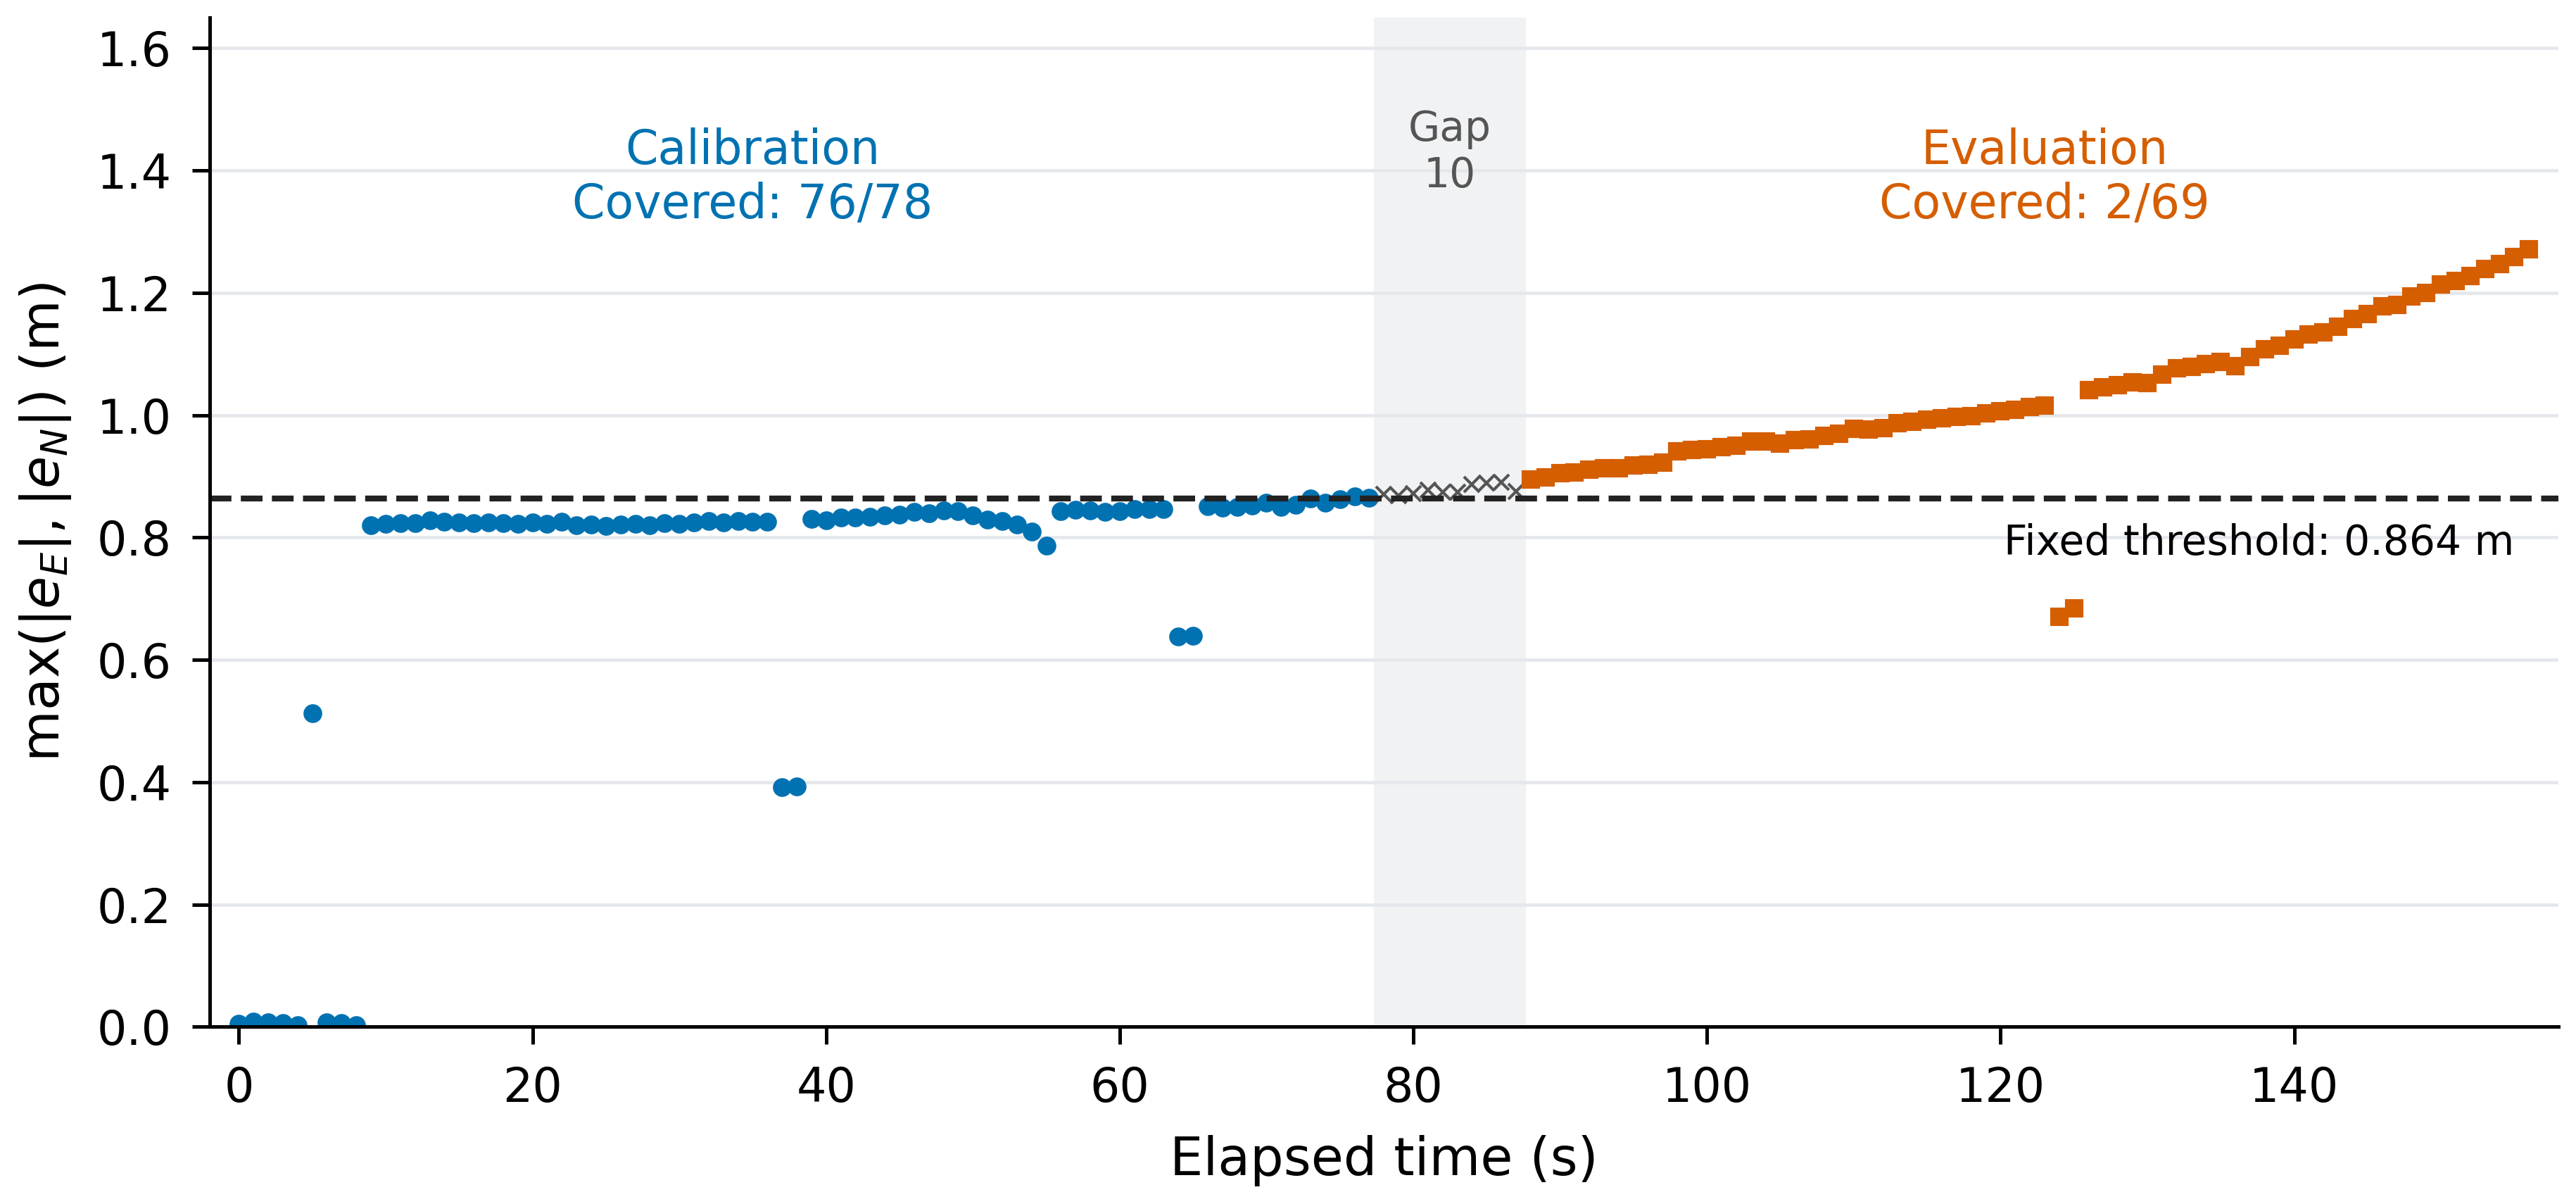
\includegraphics[width=\linewidth]{receiver_diagnostic.png}
\caption{Horizontal residual diagnostic for one stationary receiver. All 157 matched epochs are plotted, with a dashed line showing the 0.863506 m square half-width obtained from the calibration segment. Serial dependence and combined processing prevent interpreting this as online coverage performance.}\label{fig:receiver}
\end{figure}
